\documentclass{beamer}
%\documentclass[handout]{beamer}
%\documentclass[notes]{beamer}
%\documentclass[trans]{beamer}


%%%%%%%%%%%%%%%%%%%%%%%%%%%%%%%%%%%%%%%%%%%%%%%%%%%%%%%%%%%%%%%%%%%%%%%%%%%%%%%%
%%
%% Copyright 2004  by Till Tantau     <tantau@users.sourceforge.net>.
%%       and 2007  by Frédéric Haziza <daz@it.uu.se>
%%
%% In principle, this file can be redistributed and/or modified under
%% the terms of the GNU Public License, version 2.
%%
%%
%% However, you can use this file as a template to be modified for your own
%% needs. You can freely copy and modify this file as you see fit.
%%
%% Describing beamerthemeUppsala version 2007/04/04
%%
%% If you have more than three sections or more than three subsections in at least
%% one section, you might want to use the [hideallsubsections] or
%% [hideothersubsections] switch.  In this case, only the current (sub-) section is
%% displayed in the sidebar and not the full overview.
%%
%%%%%%%%%%%%%%%%%%%%%%%%%%%%%%%%%%%%%%%%%%%%%%%%%%%%%%%%%%%%%%%%%%%%%%%%%%%%%%%%


%% Options are hideallsubsections,numbers,totalnumber,withnav,sidebarshades
%\usetheme{Uppsala}
%\usetheme[hideothersubsections,numbers,sidebarshades]{Uppsala}
\usetheme[hideothersubsections,numbers,whiteblock]{Uppsala}
%\usetheme[hideothersubsections,numbers,whiteblock,mylogo]{Uppsala}
%\usetheme[hideothersubsections,numbers,menutop]{Uppsala}

\usepackage{tikz} % you only need this when using TikZ graphics

\usepackage{multimedia}
% you probably want to comment this out if not using multimedia elements

\usepackage{hyperref}

\usepackage[english]{babel} % or whatever
\usepackage[latin1]{inputenc} % or whatever

\usepackage{mathptmx}
\usepackage{helvet}
%\usepackage{courier}

\usepackage[T1]{fontenc}
% Or whatever. Note that the encoding and the font should match. If T1
% does not look nice, try deleting the line with the fontenc.

\title{\emph{Unofficial} Uppsala Theme}

\subtitle{for Beamer}

\logo{}

%% -----------------------------------------------------------
%% MISC. INFORMATION
%% -----------------------------------------------------------

\author[Fr\'ed\'eric Haziza | \emph{daz@it.uu.se}] % appears in the footline
{Fr\'ed\'eric Haziza <\texttt{daz@it.uu.se}>}

\institute[Dept. of Information Technology] % appears in the footline
{
  Department of Computer Systems\\
  Uppsala University
}

\date[2007-04-07] % appears in the bottom of the sidebar
{Sunday April $7^{th}$, 2007}


%% \logo{...}

%% This is only inserted into the PDF information catalog. Can be left out.
\subject{Beamer}

%% -----------------------------------------------------------
%% Extra ``local'' settings
%% -----------------------------------------------------------

% Comment out this, if you do not want the table of contents to pop up at
% the beginning of each (sub)section:
\AtBeginSection[]
{
  \begin{frame}<beamer> % with <beamer> => doesn't appear in handout mode
    \frametitle{Outline} %% Put the title you want, or none!
    %\tableofcontents[currentsection,currentsubsection]
    \tableofcontents[currentsection]
  \end{frame}
}

%% Unfolds piecewise element with shading.
%% Text appears, shaded, and the audience knows that somehting is coming
%% Note: if you set the number too high, the audience will try to read the 
%% text that now shows up more, and will be disturbed.
%% ``dynamic'' makes elements show gradually more and more.
\setbeamercovered{transparent=5}
%% \setbeamercovered{dynamic=5}

%% -----------------------------------------------------------

\begin{document}

\begin{frame}[plain] %% Gets the frame to fill up the page, no menu/footline
  \titlepage
\end{frame}

\begin{frame}
    \frametitle{Outline}
    \tableofcontents[currentsection]
\end{frame}

\section{Introduction}

\begin{frame}
  \frametitle{Why}

  Why use \LaTeX, when there are specialized presentations tools (OpenOffice.org Impress, Keynote, PowerPoint) available?

  \begin{itemize}
    \item{Look: The layout of mathematical formulas and program text is much nicer\ldots not to speak from ligatures in ``ordinary'' text}
    \item{Reuse of material: Going from a paper to a presentation is easy -- just use the same ``codebase''}
    \item{Portable solution: You can use whichever operating system you like}
    \item{Durable solution: usually even very old \LaTeX code can be typeset with modern installations}
  \end{itemize}

\end{frame}

\section{Cool Stuff}

\begin{frame}
  \frametitle{Mathematics}

  \begin{example}
    \begin{equation}
      \mathit{Hamming} (X,Y) = \sum_{i=1}^{n} f (x_{i}, y_{i})
    \end{equation}
  \end{example}

with $f(x,y)$ defined as follows:

  \begin{definition}
    \begin{equation}
      f(x,y)= \left\{ \begin{array}{ll}
          0 & \mbox{iff $|x-y| \leq \epsilon_{h}$,} \\
          1 & \mbox{else.}      \\
        \end{array}
      \right.
    \end{equation}
  \end{definition}

\end{frame}

\begin{frame}
  \frametitle{Piecewise Text Modification}

  \onslide<1>
    Shown on first slide.
  \onslide<2>
    Shown on second slide.
  \onslide<1>
    Shown on first slide.
    \begin{itemize}
  \onslide<2-3>
        \item Shown on the second and the third slide.
  \onslide+<3->
        \item Shown from slide 3 on.
    \end{itemize}
    Shown from slide 3 on.
  \onslide
    Shown on all slides.

    \vskip 1cm
  \onslide<4>
    \alert<4>{You get fine-grain control over which elements are visible at each time.}

\end{frame}

\begin{frame}
  \frametitle{Using Ti\textit{k}Z for Drawings}

  % The stuff for this slide is taken from the PGF Manual

  % New example using TikZ

    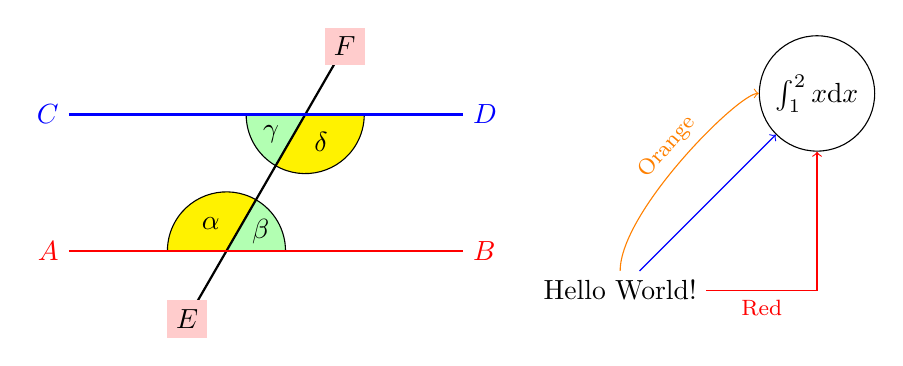
\begin{tikzpicture}
      \draw[fill=yellow] (0,0) -- (60:.75cm) arc (60:180:.75cm);
      \draw(120:0.4cm) node {$\alpha$};
      \draw[fill=green!30] (0,0) -- (right:.75cm) arc (0:60:.75cm);
      \draw(30:0.5cm) node {$\beta$};
      \begin{scope}[shift={(60:2cm)}]
        \draw[fill=green!30] (0,0) -- (180:.75cm) arc (180:240:.75cm);
        \draw (30:-0.5cm) node {$\gamma$};
        \draw[fill=yellow] (0,0) -- (240:.75cm) arc (240:360:.75cm);
        \draw (-60:0.4cm) node {$\delta$};
      \end{scope}
      \begin{scope}[thick]
        \draw (60:-1cm) node[fill=red!20] {$E$} -- (60:3cm) node[fill=red!20] {$F$};
        \draw[red] (-2,0) node[left] {$A$} -- (3,0) node[right]{$B$};
        \draw[blue,shift={(60:2cm)}] (-3,0) node[left] {$C$} -- (2,0) node[right]{$D$};
      \end{scope}
      \path (5,-0.5) node (x) {Hello World!}
      (7.5,2) node[circle,draw](y) {$\int_1^2 x \mathrm d x$};
      \draw[->,blue] (x) -- (y);
      \draw[->,red] (x) -| node[near start,below] {\footnotesize Red} (y);
      \draw[->,orange] (x) .. controls +(up:1cm) and +(left:1cm) .. node[above,sloped] {\footnotesize Orange} (y);
    \end{tikzpicture}

  \vspace*{.5cm}

  Take a look into the \href{http://path/to/beamerUppsalaExample.tex}{\alert{source code}} to see how this is done.

\end{frame}

\note{
  Example from J\"{o}rg Cassens, University of Trondheim, in his example:
  \vskip 1cm
  See \href{http://story.idi.ntnu.no/~cassens/blog/categories/20-LaTeX}{his blog on the Trondheim theme}.
}

%%%%%%%%%%%%%%%%%%%%%%%%%%%%  PFG capabilities
%% \begin{frame}
%%   \frametitle{Using Ti\textit{k}Z for Drawings -- 2}

%%   \begin{pgfpicture}{0cm}{0cm}{5cm}{2cm}
%%     \pgfputat{\pgfxy(1,1)}{\pgfbox[center,center]{Hi!}}
%%     \pgfcircle[stroke]{\pgfxy(1,1)}{0.5cm}
%%     \pgfline{\pgfxy(1.5,1)}{\pgfxy(2.2,1)}
%%      \pgfputat{\pgfxy(3,1)}{
%%      \begin{pgfrotateby}{\pgfdegree{30}}
%%        \pgfbox[center,center]{$\int_0^\infty xdx$}
%%      \end{pgfrotateby}}
%%     \pgfcircle[stroke]{\pgfxy(3,1)}{0.75cm}
%%     \pgfmoveto{\pgfxy(5,1)}
%%     \pgfcurveto{\pgfxy(6,0.5)}{\pgfxy(6,1.5)}{\pgfxy(8,1)}
%%     \pgfstroke
%%     \pgfsetdash{{3pt}{3pt}}{0pt}
%%     \pgfmoveto{\pgfxy(5,1)}
%%     \pgflineto{\pgfxy(6,0.5)}
%%     \pgflineto{\pgfxy(6,1.5)}
%%     \pgflineto{\pgfxy(7,1)}
%%     \pgfstroke
%%     \pgfmoveto{\pgfxy(9,1)}
%%     \pgfcurveto{\pgfxy(9,0)}{\pgfxy(10,0)}{\pgfxy(10,1)}
%%     \pgfcurveto{\pgfxy(10,2)}{\pgfxy(9,2)}{\pgfxy(9,1)}
%%     \pgfclosepath
%%     \pgffill
%%   \end{pgfpicture}

%% \end{frame}


%%%%%%%%%%%%%%%%%%%%%%%%%%%%  Movies capabilities
%% \begin{frame}
%%   \frametitle{Including Movies}

%%   \pgfdeclareimage[interpolate=true,width=.45\textwidth]{ccpict}{Building_On_The_Past}

%%   \begin{center}
%%     \movie[poster,externalviewer,label=mymovie]{\pgfuseimage{mypic}}{mymovie_path.mpg}
%%   \end{center}

%%   {\small
%%   To watch the movie in an external player application, click on the picture above.% or \hyperlinkmovie{mymovie}{\beamerbutton{press this button}}.

%%   The video is not included in the distribution of this PDF. To watch it, just \href{http://some/long/path/to/the/file.mpg}{\alert{fix }names, paths and all}.

%%   {\tiny Don't forget the copyright...}

%% \end{frame}

\section{Coloured Boxes}

\subsection{Alerts and Examples}

\begin{frame}
  no title
\end{frame}


\begin{frame}
  \frametitle{Alert}

  Alert boxes direct the attention of the audience.

  \begin{alertblock}{Lorem Ipsum}
    ``Lorem ipsum dolor sit amet, consectetuer.''
  \end{alertblock}
  
  \pause
  Non eram nescius, Brute, cum, quae summis ingeniis exquisitaque doctrina
  philosophi Graeco sermone tractavissent, ea Latinis litteris mandaremus, fore
  ut hic noster labor in varias reprehensiones incurreret.

  Nam quibusdam, et iis quidem non admodum indoctis, totum hoc displicet philosophari.
\end{frame}

\begin{frame}
  \frametitle{Exampleblock}

  Examples are also highlighted in a different colour, making them less obstrusive.

  \begin{example}
    ``Laoreet dolore magna ali quam erat volutprat.''
  \end{example}

  You can also use a custom title:

  \begin{exampleblock}{Comodo consequat}
    ``Ut wisi enim ad mi nim veniam, quis nostrud exerci.''
  \end{exampleblock}

\end{frame}

\subsection{Theorems and Definitons}

\begin{frame}
  \frametitle{Theorem}

  Theorems and definitions come in their own coloured boxes. A theorem:

  \begin{theorem}
    ``Lorem ipsum dolor sit amet, consectetuer.''
  \end{theorem}

  And a definition:

  \begin{definition}
    ``Laoreet dolore magna ali quam erat volutprat.''
  \end{definition}

\end{frame}


\subsection{Other Boxes}

\begin{frame}
  \frametitle{Block}

  ``UU Red'' boxes can also be used for other content you want to highlight.

  \begin{block}{Comodo consequat}
    ``Laoreet dolore magna ali quam erat volutprat.''
  \end{block}

  You can also create boxes with no header.

  \begin{block}{}
    ``Ut wisi enim ad mi nim veniam, quis nostrud exerci.''
  \end{block}

\end{frame}

\begin{frame}
  \frametitle{Beamercolorbox}

  Simple colored boxes are the least decorated way to draw attention to certain areas:\newline

  \begin{beamercolorbox}[sep=0.5em]{block title}
    ``Lorem ipsum dolor sit amet, consectetuer.''
  \end{beamercolorbox}

  \vspace*{.5cm}

  Quidam autem non tam id reprehendunt, si remissius agatur, sed tantum studium
  tamque multam operam ponendam in eo non arbitrantur.

  Erunt etiam, et ii quidem eruditi Graecis litteris, contemnentes Latinas, qui
  se dicant in Graecis legendis operam malle consumere. Postremo aliquos futuros
  suspicor, qui me ad alias litteras vocent, genus hoc scribendi, etsi sit
  elegans, personae tamen et dignitatis esse negent.

\end{frame}

\section{Conclusions}

\begin{frame}
  \frametitle{Options}

  \begin{itemize}
    \item{\textbf{Navigation:} [withnav] use the (horizontal) navigation bar right over the footline}
    \item{\textbf{Page numbers:} [numbers|totalnumber] will include the number of the current slide in the footline (along with the total number)}
    \item{\textbf{Section overview:} [hideallsubsections|hideothersubsections]}
    \item{\textbf{Shades:} [sidebarshades] use shades (darker red boxes around the active section)}
  \end{itemize}

    \begin{example}[My favorite]
      {\footnotesize{
	  $\backslash$usetheme[hideothersubsections,numbers,sidebarshades]\{Uppsala\}
      }}
  \end{example}

\end{frame}

\begin{frame}
  \frametitle{Options -- Wish list}
  Not yet implemented:
  \begin{itemize}
    \item{\textbf{Sidebar colour:} [red|grey] sets the background colour accordingly}
    \item{\textbf{Top menu:} [topmenu] new version, better contrast, more adequate}
    \item{\textbf{Minimal:} [minimal] new version, minimal information, sober}
  \end{itemize}

  \begin{alertblock}{Note}
    No guarantees are given of any kind. Especially if you use the uu font or
    color theme outside the Uppsala theme.
    \vskip 5mm 
    I would appreciate help more than destructive critics, since I am not a
    \LaTeX\ expert.
  \end{alertblock}
  

\end{frame}

\begin{frame}
  \frametitle{Conclusions}

  \begin{itemize}
    \item Theme based on PaloAlto theme that comes with Beamer
    \item Suited for (long) scientific talks with UU style
    \item The colours used in this theme are based on  ``UU red'' plus darker shades
    \item The hide[all|other]subsections switch is useful if you are having (too) many (sub-) sections
    \item Feedback appreciated: \href{mailto:daz@it.uu.se}{\texttt{daz@it.uu.se}}
    \item Non official $\Rightarrow$ I could use some help
  \end{itemize}
\end{frame}

\begin{frame}[plain]
  \begin{centering}
    \pgfimage[height=\textheight]{uppsala_logo}
    \par
  \end{centering}
\end{frame}

\end{document}
